
\documentclass[12pt]{article}

\usepackage{Homework}
% \usepackage{kbordermatrix}
\usepackage{blkarray, bigstrut}
\newcommand{\matindex}[1]{\mbox{\scriptsize#1}}% Matrix index

% Creates the header and footer.
\pagestyle{fancy}
\fancyhead[l]{Michael Hoon, $1006617$}
\fancyhead[c]{40.012 MSO 2.0 Homework 1}
\fancyhead[r]{\today}
\fancyfoot[c]{\thepage}
\renewcommand{\headrulewidth}{0.2pt} %Creates a horizontal line underneath the header
\renewcommand{\footrulewidth}{0.2pt}
\setlength{\headheight}{15pt} %Sets enough space for the header
\newcommand{\HRule}[1]{\rule{\linewidth}{#1}}
\newcolumntype{L}{>{\centering\arraybackslash}m{4cm}}


\begin{document}

% \title{Another fancyhdr demo}
% \author{\texttt{tex.stackexchange} \textit{et al}}
% \maketitle
% \newpage


\title{ \normalsize \textsc{} 
        \\ [2.0cm]
		\HRule{1.5pt} \\
		\LARGE \textbf{\uppercase{40.012 Manufacturing and Service Operations 2.0} 
        \HRule{2.0pt} \\ [0.6cm]
        \LARGE{Homework 1} \vspace*{10\baselineskip}}
		}
\date{\today}
\author{\textbf{Michael Hoon} \\ 1006617}


\maketitle 

\newpage

\section*{Question 1}

We have a total of $N$ interconnected nodes in a network repreentation of the cat-eat-mouse situation, with 2 of those nodes being occupied by both the cat and the mouse. If we consider that they move independently of one another, then each has a total of $N-1$ choices to choose from for the next discrete time step. We first define $X_n$ as the state of the system at time $n$: \begin{align*}
    X_n = \begin{cases}
        0, \quad \text{if mouse dead} \\ 
        1, \quad \text{if mouse alive} \\ 
    \end{cases}
\end{align*} The state space here is $\mathcal{S} = \{0, 1\}$, as the mouse can only be dead or alive at any moment. Now, we consider the transition probabiliity matrix. For the trivial cases, we assume here that the mouse is mortal and will not revive after being consumed by the cat, so the transition from state 0 to itself $p_{0,0}$ will have a probability of 1, and similarly the transition probability from state 0 to 1 $p_{0,1}$ is 0. To consider the case where the mouse gets consumed at the next time step, we need to find the probability that they both choose the same node. There are only $N-2$ possibilities here as mentioned earlier, thus the transition probability for a total of $(N-1)\times(N-1)$ possible arrangements is $p_{1,0} = (N-2) / (N-1)(N-1)$. The final case is just the complement of this, so $p_{1,1} = 1 - (N - 2) / (N-1)(N-1)$. The transition matrix is thus \begin{equation}
        P_{i, \; j} = \begin{blockarray}{ccc}
        & \matindex{0} & \matindex{1} \\ 
            \begin{block}{c[cc]}
                \matindex{0} & 1 & 0 \\ 
                \matindex{1} & \frac{N-2}{(N-1)^{2}} & 1 - \frac{N-2}{(N-1^{2})} \\
            \end{block}
        \end{blockarray}
\end{equation} The transition diagram is given in Figure below. 

\begin{figure}[h]
    \centering
    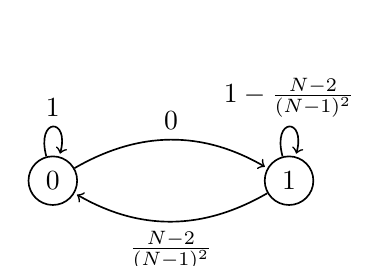
\begin{tikzpicture}[->, shorten >=1pt, auto, node distance=3cm, semithick]

      % Define states
      \node[circle, draw] (0) {0};
      \node[circle, draw, right of=0] (1) {1};

      % Define transitions
      \path (1) edge [loop above] node {$1-\frac{N-2}{(N-1)^{2}}$} (1)
            (1) edge [bend left] node [below] {$\frac{N-2}{(N-1)^{2}}$} (0)
            (0) edge [bend left, above] node {$0$} (1)
            (0) edge [loop above] node {1} (0);

    \end{tikzpicture}
    \caption{Transition Diagram for Cat and Mouse Problem}
    \label{fig:1-transition_diagram}
\end{figure}

\section*{Question 2}

First, we define the state of the system on the $n^{\text{th}}$ day \begin{equation}
    X_n = \begin{cases}
        s, \quad \text{if day } n \text{ is sunny}\\
        r, \quad \text{if day } n \text{ is rainy}
    \end{cases}
\end{equation} We then define today's state of the system as a pair $(W_{n-1}, W_n)$ with $W_{n-1}$ and $W_n$ representing yesterday's and today's weather respectively. Since we only have two weather conditions, Sunny or Rainy, the state space here has 4 possible combinations, $\mathcal{S} = \{(s,s), (s,r), (r,s), (r,r)\}$. Next, we calculate the transition probabilities. The cases defined in the question are \begin{enumerate}
    \item $(s,s) \to (s,s)$: $p = 0.8$
    \item $(s,s) \to (s,r)$: $p = 1 - 0.8 = 0.2$
    \item $(s,r) \to (r,s)$: $p = 0.5$
    \item $(s,r) \to (r,r)$: $p = 1- 0.5 = 0.5$
    \item $(r,s) \to (s,s)$: $p = 0.75$
    \item $(r,s) \to (s,r)$: $p = 1-0.75 = 0.25$
    \item $(r,r) \to (r,s)$: $p = 0.4$
    \item $(r,r) \to (r,r)$: $p = 1-0.4=0.6$
\end{enumerate} With this, we can construct the transition matrix as follows, following the order of the state spaces in $\mathcal{S}$: \begin{equation}
        P_{i, \; j} = \begin{blockarray}{ccccc}
                & \matindex{(s,s)} &\matindex{(s,r)} &\matindex{(r,s)} &\matindex{(r,r)} \\ 
            \begin{block}{c[cccc]}
                \matindex{(s,s)} & 0.8 & 0.2 & 0 & 0 \\ 
                \matindex{(s,r)} & 0 & 0 & 0.5 & 0.5 \\ 
                \matindex{(r,s)} & 0.75 & 0.25 & 0 & 0 \\ 
                \matindex{(r,r)} & 0 & 0 & 0.4 & 0.6 \\ 
            \end{block}
        \end{blockarray}
\end{equation}

\section*{Question 3}

We first define the state $X_n$ be the number of bugs in the program just before running it for the $n^{\text{th}}$ time. Here, we have $X_n = k$. The state space is infinite, i.e. $\mathcal{S} = \{0,1,2,\dots\}$. To determine the transition probabilities, we need to consider the two given probabilities $p_k$ and $b_i, \; \forall i = 0, 1, 2$. Consider the following cases: \begin{enumerate}
    \item The program is ran and a bug is introduced with probability $p_k$. \begin{itemize}
        \item If a bug is discovered, it is fixed. No new bugs are introduced with probability $b_0$. $k' = k - 1$
        \item One new bug is introduced with probability $b_{1}$. $k' = k$
        \item Two new bugs are introduced with probability $b_{2}$. $k' = k + 1$
    \end{itemize}
    \item No bug is discovered with probaility $(1-p_k)$. 
\end{enumerate}

\noindent With this, we can determine the transition probabilities $p_{i,j}$, which is the probability of transitioning from state $i$ to state $j$. First, consider the trivial case where $i=j=0$. $p_{0,0} = 1$ since no bugs are discovered, and no new bugs can be introduced. For $i > 0$, we have 3 cases as defined previously: \begin{enumerate}
    \item $j = i - 1$, $p_{i, \; i-1} = p_i \cdot b_{0}$. Here, we discover a bug and introduce 0 new bugs, reducing the number of bugs in the next state by 1 since it is fixed after discovery. 
    \item $i = j = 1$, $p_{i,\;i} = (1-p_i) + p_i \cdot b_{1}$. Here, the state \textbf{remains the same} and we can have two possibilities of this occurring: one where we do not discover new bugs on a run, and another where we discover a bug, fix it, and introduce only 1 new bug. 
    \item $j = i + 1$, $p_{i, \; i+1} = p_i \cdot b_{2}$. Here, the only case where we can have one more bug than the previous state is to discover a bug, and then introduce 2 new bugs after fixing it. 
\end{enumerate}

\noindent These probabilities are based on the fact that the bug discovering and bug introducing process are independent of each other. The transition probabilities can thus be represented by: \begin{equation}
    p_{i, \j} = \begin{cases}
        1, \quad & i = j = 0 \\ 
        p_i\cdot b_{0}, \quad & i, \; j = i - 1 \\ 
        (1-p_i) + p_i \cdot b_{1}, \quad & i=j  \\ 
        p_{i} \cdot b_{2}, \quad & i, \; j = i + 1 \\ 
        0, \quad & \text{otherwise}
    \end{cases}
\end{equation} We can represent the transition probability matrix as follows: \begin{equation}
        P_{i, \; j} = \begin{blockarray}{cccccc}
                & \matindex{0} & \matindex{1} & \matindex{2} &\matindex{3} &\matindex{\dots} \\ 
            \begin{block}{c[ccccc]}
                \matindex{0} & 1 & 0 & 0 & 0 & \dots \\ 
                \matindex{1} & p_{1}b_{0} & (1-p_{1}) + p_{1}b_{1} & p_{1} b_{2} & 0 & \dots \\ 
                \matindex{2} & 0 & p_{2}b_{0} & (1-p_{2}) + p_{2}b_{1} & p_{2}b_{2} & \dots \\ 
                \matindex{3} & 0 & 0 & p_{3}b_{0} & (1-p_{3}) + p_{3}b_{1} & \dots \\ 
                \matindex{\vdots} & \vdots & \vdots & \vdots & \vdots & \ddots \\
            \end{block}
        \end{blockarray}
\end{equation} To show that $\{X_n, n \geq 1\}$ is a DTMC, we need to validate the two properties of memorylessness and time-invariance. Since we are already given in the question that the bug discovering and bug introducing processes are independent of the past runs and each other, we have already satisfied the Markov property and can conclude that it is indeed a DTMC. 

\section*{Question 4}

Let $X_n$ be the age of the light bulb that is on at time $n$. Here, we have an infinite state space $\mathcal{S} = \{0, 1, 2, \dots\}$. We are given that $X_n = 0$ if a failure has taken place at time $n$, and $Z_i$ is the lifetime of the $i^{\text{th}}$ bulb, where $\{Z_i, i\geq 1\}$ is a sequence of iid DRV: \begin{equation}\label{eq:4-lifetime}
    \mathbb{P}\{Z_i = k\} = p_k, \quad \forall k = 1, 2, \dots
\end{equation} We need to identify the transition probabilities for each state change. Consider a few cases here to identify a trend: \begin{enumerate}
    \item For a state change from $0 \to 0$, $p_{0, \; 0}$: Here, the age is 0 and does not change. The only case where this can happen is that for a lightbulb $i$, the lifetime is 1 unit, and it fails and gets replaced by a new lightbulb with age 0. Thus, $p_{0, \; 0} = \mathbb{P}\{Z_i = 1\} = p_{1}$. 
    \item For $0 \to 1$, $p_{0, \; 1}$ indicates that the light bulb did not fail in the next discrete time interval. The transition probability here is just the complement of the previous case, $(1 - p_{1})$. However, for transitions from $0 \to 2 / 3 / 4 \dots$ and beyond, this is not possible. 
    \item For any $X_n = k$, we can see that $X_{n+1}$ can only be $0$ or $k + 1$, where a new lightbulb is introduced here, or the same lightbulb increases in age by 1 unit. Thus, we have \begin{equation}\label{eq:4-xn+1}
        X_{n+1} = \begin{cases}
            0, \quad & \text{if original bulb fails} \\ 
            k + 1 \quad & \text{otherwise}
        \end{cases}
    \end{equation}
    \item Let us consider the case where $X_{n+1} = 0$ (i.e. $p_{k, \; 0}$), given that the previous bulb has age $k$ prior to failure (new bulb introduced). The only case where this can happen is if the lifetime of the bulb is more than $k$ units, where the probability of this happening is $p_{k+1}$ based on Equation \ref{eq:4-lifetime}, given that it has a previous age of $k$ units. We need to introduce conditional probability here, where \begin{align*}
        p_{k, \; 0} &= \mathbb{P}(X_{n+1} = 0 \vert X_n = k) \\ 
        &= \mathbb{P}(Z_i = k + 1 | Z_i > k) \\ 
        &= \frac{ \mathbb{P}\left((Z_i = k + 1) \cap (Z_i > k) \right)}{ \mathbb{P}(Z_i > k)} \\ 
        &= \frac{ \mathbb{P}\left(Z_i = k + 1\right)}{ \mathbb{P}(Z_i \geq  k+1)} \\ 
        &= \frac{p_{k+1}}{ \sum_{i=k+1}^{\infty} p_i}
    \end{align*} 
    \item We now consider the case where $X_{n+1} = k+1$, where the light bulb does not fail and ages by 1 unit. Here, the transition probability is $p_{k, \; k+1}$, and is just the complement of $p_{k, \; 0}$: \begin{align*}
        p_{k, \; k+1} &= \mathbb{P}(X_{n+1} = k + 1 | X_n = k) \\ 
        &= 1 - p_{k, \; 0} \\ 
        &= 1 - \frac{p_{k+1}}{ \sum_{i=k+1}^{\infty} p_i}
    \end{align*}
    \item Lastly, we need to consider the case of $p_{k, \; k}, \; \forall k > 0$. This is not possible as there are only two cases of $X_{n+1}$ from Equation \ref{eq:4-xn+1}, and the age of the lightbulb cannot remain the same. Similarly, the other cases are also not possible as mentioned in Point 2. 
\end{enumerate}

\noindent The resulting piecewise function for the transition probabilities for all possibilities detailed earlier is: \begin{equation}
    p_{i, \;j} = \begin{cases}
        \displaystyle\frac{p_{k+1}}{ \sum_{m=k+1}^{\infty} p_m}, \quad & \text{for } i = k, \; j = 0 \\ 
         1 - \displaystyle\frac{p_{k+1}}{ \sum_{m=k+1}^{\infty} p_m}, \quad & \text{for } i = k, \; j = i + 1 \\ 
         0, \quad \text{otherwise}
    \end{cases}
\end{equation} Similarly, the transition probability matrix is shown below: \begin{equation}
        P_{i, \; j} = \begin{blockarray}{cccccc}
                & \matindex{0} & \matindex{1} & \matindex{2} &\matindex{3} &\matindex{\dots} \\ 
            \begin{block}{c[ccccc]}
                \matindex{0} & p_{1} & 1-p_{1} & 0 & 0 & \dots \\ 
                \matindex{1} & \frac{p_{2}}{ \sum_{i=2}^{\infty} p_i} & 0 & 1-\frac{p_{2}}{ \sum_{i=2}^{\infty} p_i} & 0 & \dots \\ 
                \matindex{2} & \frac{p_{3}}{ \sum_{i=3}^{\infty} p_i} & 0 & 0 & 1-\frac{p_{3}}{ \sum_{i=3}^{\infty} p_i} & \dots \\ 
                \matindex{3} & \frac{p_{4}}{ \sum_{i=4}^{\infty} p_i} & 0 & 0 & 0 & \dots \\ 
                \matindex{\vdots} & \vdots & \vdots & \vdots & \vdots & \ddots \\
            \end{block}
        \end{blockarray}
\end{equation} To show that $\{X_n, n\geq 1\}$ is a DTMC, we need to verify the Markov properties of memorylessness and time invariance. The transition probabilities $p_{i, \; j}$ only depend on the current state and not on any previous states, and is clearly time invariant as it applies for all units of time. Hence, it is a DTMC. 

\section*{Question 5}

Let $Y_n$ be the number of people who board the bus at stop $n$. We have that $\{Y_n, n\geq 0\}$ is an iid sequence of RVs with common PMF \begin{equation}
    \mathbb{P}\{Y_n = k\} = p_k, \quad k = 0, 1, 2, \dots 
\end{equation} Here, the state space is infinite $\mathcal{S} = \{0, 1, 2, \dots\}$. Let $X_n$ be the number of passengers on the bus when it leaves the $n^{\text{th}}$ stop. Each person that is currently on the bus will alight at stop $n$ with probability $p$. Since there are $X_n$ possible total number of passengers that can alight, each with probability $p$ \textbf{independently}, then the number of passengers that alight at the $n^{\text{th}}$ stop $A_n$ is $A_n \sim \text{Binom}(X_{n}, p)$, and follows a Binomial distribution. Let's consider that there are $i$ passengers at the $n^{\text{th}}$ stop, i.e. $X_n = i$. \\ 

\noindent To find the transition probabilities, we need to consider the next state $X_{n+1}$, i.e. $ \mathbb{P}(X_{n+1} = j | X_n = i)$. Then, $A_n \sim \text{Binom}(i, p)$, and the number of passengers that board has PMF $p_k$. Note that $X_{n+1} = X_n - A_n + Y_{n+1}$. Here, we need to use the law of total probability to express the next state probability conditioned onto $Y_{n+1}$, the number of passengers who board at stop $n+1$. Since we have an infinite capacity bus, we use the formula for Law of Total Probability to obtain: \begin{align*}
    \mathbb{P}(A) &= \sum_{n} \mathbb{P}(A | B_n) \cdot \mathbb{P}(B_n) \\ 
    \mathbb{P}(X_{n+1} = j | X_n = i) &= \sum_{k=0}^{\infty} \mathbb{P}((X_{n+1} = j | X_n = i) | Y_{n+1} = k) \cdot \mathbb{P}(Y_{n+1} = k | X_n = i) \\ 
    &= \sum_{k=0}^{\infty} \mathbb{P}(X_{n+1} = j | X_n = i, Y_{n+1} = k) \cdot \mathbb{P}(Y_{n+1} = k) \\ 
    & \quad (\text{since } Y_{n+1} \text{ is independent of } X_n)
\end{align*} Now, we need to simplify the expressions for the probabilities above. Clearly, $ \mathbb{P}(Y_{n+1} = k) = p_k$, the number of people who board the bus at stop $n+1$. Next, we need to determine the conditional probability $ \mathbb{P}(X_{n+1} = j | X_n = i, Y_{n +1} = k)$, which is the probability that there are $j$ passengers on the bus after stop $n+1$, given that there were $i$ passengers on the bus before stop $n+1$ and $k$ new passengers boarded the bus at stop $n+1$. Since we have that $X_n = i$, $X_{n+1} = j$ and $Y_{n+1} = k$, then \begin{align*}
    X_{n+1} &= X_n - A_n + Y_{n+1} \\ 
    j &= i - A_n + k \\ 
    A_n &= i - j + k
\end{align*} Trivially, the number of passengers who alight can only range between 0 and $i$. We consider the following cases: \begin{enumerate}
    \item $A_n < 0$: $i - j + k < 0 \Longrightarrow j > i + k$. This case is impossible and hence the probability of this occurring is 0. 
    \item $A_n > i$: $i - j + k > i \Longrightarrow k > j$. This case is also impossible and hence the probability of this occuring is 0. 
    \item Acceptable range: $0 \leq A_n \leq i$: $0 \leq i - j + k \leq i \Longrightarrow k \leq j \leq i+k$. 
\end{enumerate} 

\noindent Here, the probability of exactly $i - j + k$ passengers alighting follows a Binomial distribution described by $A_n$, so \begin{equation}
    \mathbb{P}(A_n = i - j + k | X_n = i) = \binom{i}{i - j + k}p^{i - j + k}(1-p)^{j - k}
\end{equation} and thus \begin{equation}
    \mathbb{P}(X_{n+1} = j | X_n = i, Y_{n+1}) = \begin{cases}
        0, \quad & j > i + k \\ 
        0, \quad & k > j \\
        \displaystyle\binom{i}{i-j+k}p^{i - j + k}(1-p)^{j - k}, \quad & k \leq j \leq i + k  
    \end{cases}
\end{equation} Now, we can find the transition probability, which is \begin{align*}
    \mathbb{P}(X_{n+1} = j | X_n = i) &= \sum_{k=0}^{\infty} \mathbb{P}(X_{n+1} = j | X_n = i, Y_{n+1} = k) \cdot \mathbb{P}(Y_{n+1} = k) \\ 
    &= \sum_{k=0}^{\infty} \left( \displaystyle\binom{i}{i-j+k}p^{i - j + k}(1-p)^{j - k} \right) \cdot p_k
\end{align*} To determine the limits of the summation operator, we need to consider the acceptable range of passengers alighting. Based on points 1 and 2 above, we need the inequalities $j \leq i + k$ and $k \leq j$ for the solution to be feasible. Reordering in terms of $k$, we get the following limits of summation: $k \geq j - i$ and $k \leq j$. We also need to consider that the lower limit must be $k \geq 0$, so we take the absolute value instead: $k \geq \vert j - i \vert$. Putting this together, we have an expression for the transition probability: \begin{equation}\label{eq:4-pij}
     p_{i,\; j} = \mathbb{P}(X_{n+1} = j | X_n = i) = \sum_{k=\vert j - i \vert}^{j} \left( \displaystyle\binom{i}{i-j+k}p^{i - j + k}(1-p)^{j - k} \right) \cdot p_k \\ 
\end{equation} The transition matrix will look something like (ignore first) \begin{equation}
    P_{i, \; j} = \begin{blockarray}{cccccc}
                    & \matindex{0} & \matindex{1} & \matindex{2} &\matindex{3} &\matindex{\dots} \\ 
                \begin{block}{c[ccccc]}
                    \matindex{0} & p_{1} & 1-p_{1} & 0 & 0 & \dots \\ 
                    \matindex{1} & \frac{p_{2}}{ \sum_{i=2}^{\infty} p_i} & 0 & 1-\frac{p_{2}}{ \sum_{i=2}^{\infty} p_i} & 0 & \dots \\ 
                    \matindex{2} & \frac{p_{3}}{ \sum_{i=3}^{\infty} p_i} & 0 & 0 & 1-\frac{p_{3}}{ \sum_{i=3}^{\infty} p_i} & \dots \\ 
                    \matindex{3} & \frac{p_{4}}{ \sum_{i=4}^{\infty} p_i} & 0 & 0 & 0 & \dots \\ 
                    \matindex{\vdots} & \vdots & \vdots & \vdots & \vdots & \ddots \\
                \end{block}
            \end{blockarray}
\end{equation} To prove that $\{X_n, n \geq 0\}$ is a DTMC, we need to satisfy the Markov properties. It is memoryless as $X_{n+1}$, the number of passengers as it leaves the $(n+1)^{\text{th}}$ stop, only depends on the number of passengers as it leaves the $n^{\text{th}}$ stop $X_n$, the number of passengers that alight at the $n^{\text{th}}$ stop $A_n$, and the number of passengers who board at the $(n+1)^{\text{th}}$ stop $Y_{n+1}$. It is also time-invariant as the transition probabilities remain the same across all bus stops in the state space $\mathcal{S}$, from equation \ref{eq:4-pij}. 

% \newpage

% \bibliographystyle{plain}
\bibliography{refs3}

\end{document}
